\chapter*{GPT-3 : Part 2 - Demonstration}
\label{chap:demonstration}
\thispagestyle{fancy}
\addcontentsline{toc}{chapter}{\nameref{chap:demonstration}}

\hspace{0.5cm} When GPT-3 was released the media was hyped. Many examples floated around the internet which brought to spotlight some of its impressive capabilities. For instance, here's is an excerpt from an article written by GPT-3 on the \emph{Importance of being on Twitter} \cite{mitrvw:nlmsgcm}:

\begin{quote}
    It is a curious fact that the last remaining form of social life in which the people of London are still interested is Twitter. I was struck with this curious fact when I went on one of my periodical holidays to the sea-side, and found the whole place twittering like a starling-cage. I called it an anomaly, and it is.
    
    I spoke to the sexton, whose cottage, like all sexton's cottages, is full of antiquities and interesting relics of former centuries. I said to him, "My dear sexton, what does all this twittering mean?" And he replied, "Why, sir, of course it means Twitter." "Ah!" I said, "I know about that. But what is Twitter?" ...
\end{quote}

A tweet shows how GPT-3 is able to generate code from description, another one on the right depicts GPT-3's intricate pattern matching caliber \cite{twt:1282676454690451457} \cite{twt:1285410751092416513}.

\begin{figure}[!htbp]
    \centering
    \begin{minipage}{0.45\textwidth}
        \centering
        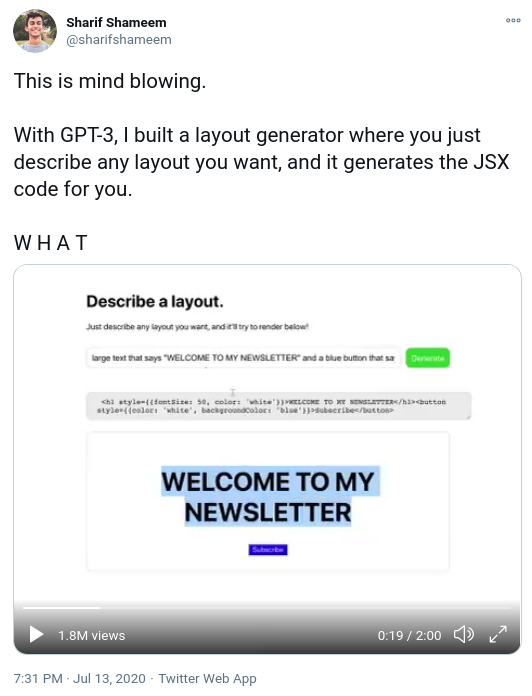
\includegraphics[height=\textwidth]{layout_gen_gpt3.png}
        \caption[GPT-3 Layout Generator]{\centering GPT-3 Layout Generator}
        \label{fig:lytgen}
    \end{minipage}\hfill
    \begin{minipage}{0.45\textwidth}
        \centering
        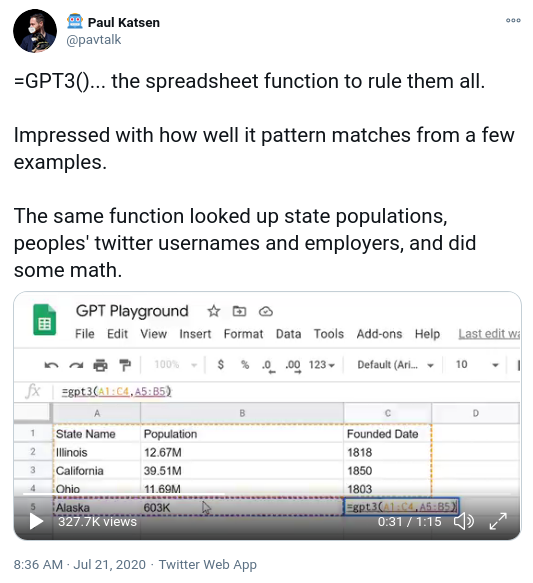
\includegraphics[height=\textwidth]{spreadsheet_func_gpt3.png}
        \caption[GPT-3 Spreadsheet function]{\centering GPT-3 Spreadsheet function}
        \label{fig:spsfnc}
    \end{minipage}
\end{figure}

\vspace*{\fill}